\section{Results}
\label{sec:results}

We report results on ARC-AGI-1 here, with early results for ARC-AGI-2 and ARC-AGI-3 in Appendix~\ref{app:tracks}. Table~\ref{tab:tests} gives the share learned on the stream, $L$, and the share saved on the two tests, $S_{\mathrm{seen}}$ and $S_{\mathrm{held}}$, for GLM-5.3 Flash (G) and Qwen3.5-9B (Q). Figure~\ref{fig:plane} plots absolute and relative solve rates, and budget used and share saved, $S_{\mathrm{seen}}$ and $S_{\mathrm{held}}$. Figure~\ref{fig:notes-weights} plots each method's share solved and budget by task visit. We also test GPT-6 Luna at high effort in prime-agent \citep{karten2026primeagent}, hermes-agent \citep{nous2026hermesagent} and openclaw \citep{openclaw2026}, see Figure~\ref{fig:plane-luna}. Shares saved below are read at the lower right quadrants of Figures~\ref{fig:plane} and~\ref{fig:plane-luna}.

\begin{figure}[t]
\centering
\includegraphics[width=\linewidth]{\hoped{figures/notes-weights}.pdf}
\caption{At one user. Bands show 95\% intervals over task resamples. GLM's budget is averaged only over instances it solves.}
\label{fig:notes-weights}
\end{figure}

\begin{figure}[t]
\centering
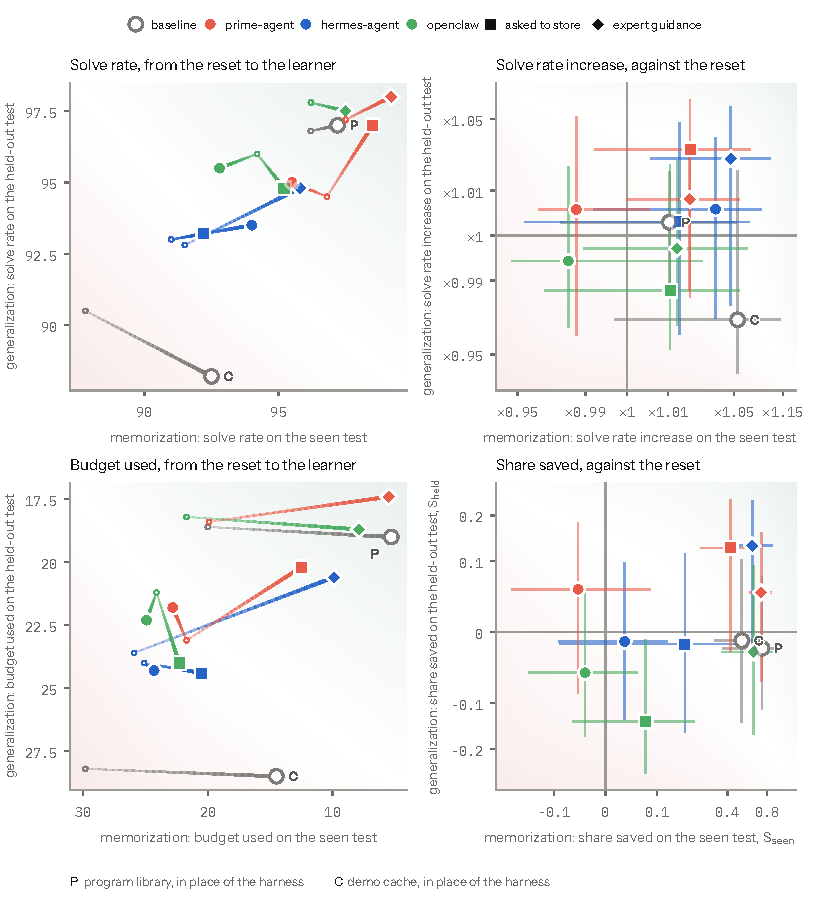
\includegraphics[width=\linewidth]{figures/plane-luna.pdf}
\caption{GPT-6 Luna at high effort, as in Figure~\ref{fig:plane}. Appendix~\ref{app:results} gives every effort.}
\label{fig:plane-luna}
\end{figure}

\paragraph{Baselines.}
Against the stateless floors (QC\textsubscript{0}, GC\textsubscript{0}), the demo-cache floors (QC, GC) saved $S_{\mathrm{seen}} = 0.37$ [0.26, 0.51] and 0.44 [0.34, 0.57] respectively (Figure~\ref{fig:plane}), which is the saving from not paying for the demonstrations twice. On new tasks there was nothing to replay, so the saving was nil, with $S_{\mathrm{held}} = -0.01$ and $-0.02$. The program libraries (QP, GP) beat the demo caches by a wide margin on the seen test, with $S_{\mathrm{seen}} = 0.65$ [0.46, 0.86] and 0.81 [0.59, 1.00] respectively (Appendix~\ref{app:plane-baselines}), but they also saved nothing measurable in $S_{\mathrm{held}}$, with 0.03 [$-0.02$, 0.09] and 0.05 [$-0.06$, 0.14]. This is to be expected, as a program verified on the demonstrations of one task does not solve another.

\paragraph{Harnesses as shipped.}
Left to their own prompting, only G saved measurably on either test across three harnesses, four models, and GPT-6 Luna's three efforts (Figures~\ref{fig:plane} to~\ref{fig:plane-luna} and Appendix~\ref{app:tracks}). This was despite the instructions at the start of every session stating that tasks recur with fresh inputs, that each instance starts a new conversation, and that each demonstration or incorrect attempt costs one (Appendix~\ref{app:prompts}). Neither harness (Q, G) beat its demo-cache floor (QC, GC; Figure~\ref{fig:plane}). Likewise, Q's persistence saved nothing measurable against its reset, with $S_{\mathrm{seen}} = -0.01$ [$-0.04$, 0.03] and $S_{\mathrm{held}} = -0.01$ [$-0.05$, 0.03] (Figure~\ref{fig:plane}), but G's saved a bit, with $S_{\mathrm{seen}} = 0.25$ [0.17, 0.33] over three runs. Further, neither expert guidance (QE) nor asking the harness to save liberally (QA, Appendix~\ref{app:ablations}) saved Q measurably, nor did the teacher's notes (QT and QTE), despite the teacher leaving 106 and 104 notes and files, respectively. For all of these, $S_{\mathrm{seen}}$ lies between 0.01 and 0.06, and $S_{\mathrm{held}}$ between $-0.02$ and 0.03. Even G, which solved nearly every instance, still spent \sbGlmHCost{}\% of the budget per solved instance after every task had been met, against \sbGlmHzeroCost{}\% for G\textsubscript{0} (Figure~\ref{fig:notes-weights}, right), where perfect memory spends nothing. We investigated this: G kept a rule in words for every task in prime-agent's store, but the harness only showed six entries per instance, chosen before the task was known, so the rule reached G on only 40 of 154 returns (Appendix~\ref{app:persist-glm}). To investigate further, we also read what each of the three harnesses (H) stored with GPT-6 Luna driving (Figure~\ref{fig:plane-luna} and Appendix~\ref{app:persist}). prime-agent kept an entry for later sessions only when the agent saved it as global, as its prompt explained, and the agent never did. hermes-agent loaded its skills on every return, but they held general advice which did not affect spend. openclaw never promoted a memory at all, and an earlier correct answer never came back on any of its returns. None of the three harnesses kept the demonstrations it paid for, each buying 2.3 to 3.9 pairs per instance where the demo-cache floor bought 1.4 to 2.6. This suggests that the harnesses' own prompting is not well suited to this domain.

\paragraph{Asking to store.}
Given that several harnesses were failing to store anything, we tried explicitly prompting the harnesses after every verdict to save very liberally anything that could help with the task's future instances (H-A). However, this only made a measurable difference for prime-agent on the seen test. With GPT-6 Luna driving, it saved $S_{\mathrm{seen}} = 0.42$ [0.29, 0.55], while hermes-agent's 0.18 [$-0.01$, 0.39] and openclaw's 0.07 [$-0.02$, 0.17] were within noise of nothing (Figure~\ref{fig:plane-luna}). With GLM driving, it saved 0.26 [0.13, 0.39] (GA), and with Qwen it was also within noise, at 0.02 [$-0.02$, 0.07] (QA). Overall, the harnesses still gained little from persistence, despite the prompting.

\paragraph{Expert guidance.}
To see if we could push the performance of the harnesses further, we added ``expert'' guidance, which explicitly told the harness to write Python programs to solve the tasks, verify each program against the demonstrations, save it for its task and reuse it. With it, GE saved $S_{\mathrm{seen}} = 0.74$ [0.64, 0.84] and the three harnesses on GPT-6 Luna (H-E) saved 0.62 to 0.72 (Figure~\ref{fig:plane-luna}). Q memorized only when the teacher wrote its notes and both were given the guidance (QETE), with $S_{\mathrm{seen}} = 0.34$ [0.26, 0.42]. This shows that the harnesses were fully capable of performing well, and that the failure was a combined lack of judgment of the model and failure of the harness prompts to encourage the correct behavior in this domain.

\paragraph{Generalization.}
The Re-ARC generators derive all 400 ARC-AGI-1 training rules from one library of 160 primitive functions \citep{hodel2024rearc}, and therefore the seen and held-out tasks both share the same building blocks. A harness which learns to abstract and store these shared building blocks during the stream could then theoretically use these to improve performance on the held-out tasks. Despite this, none of the harness methods generalized measurably (Table~\ref{tab:tests}, Figure~\ref{fig:plane-luna} and Appendix~\ref{app:bench}). This includes QETE, in which GLM, given the expert guidance, played the whole stream and wrote every program and note, solving 98\% of the instances, which Qwen failed to put to use on the held-out test. In contrast, training the weights generalized measurably, with DAgger (QDE) saving $S_{\mathrm{held}} = 0.29$ [0.23, 0.35], half its $S_{\mathrm{seen}} = 0.57$ [0.48, 0.67]. Untrained, Qwen actually struggled to use the harness at all, solving only 18 of the 100 held-out tasks in prime-agent (Q\textsubscript{0}) against 31 in the stateless loop (QC\textsubscript{0}). As a result, part of what DAgger learned was simply to drive the harness. This quirk is visible in Figure~\ref{fig:plane} (top left), where the harness method resets sit below those of QC and QP. Providing expert guidance to the untrained Qwen in the harness offsets some of this degradation, lifting its held-out solves from 13--26 to 22--33 per play (Appendix~\ref{app:told}). DAgger, however, solved 47 to 52, beyond both, and so also learned something fundamental about ARC itself, on top of learning to drive the harness and distilling the expert guidance.

\paragraph{More users.}
At two and four users (QDE(2) and QDE(4)), each bringing 25 tasks of their own, DAgger's adapter trained on the games of 50 and 100 tasks. On the held-out test it then saved $S_{\mathrm{held}} = 0.40$ at two users and 0.39 at four (Figure~\ref{fig:plane}). Seemingly, DAgger reached diminishing returns for generalization beyond two users. The full training dynamics are shown in Appendix~\ref{app:trained}.
\FloatBarrier
